\chapter{Hashing Organization}

\section{Table Organizations Based on a Key}
The \textbf{goal} of a table organization based on a key is to allow the retrieval of a record with a specified key value in as few accesses as possible, 1 being the optimum. To
this end, a mapping from the set of keys to the set of records is defined, and can be implemented in two ways:
\begin{enumerate}
    \item \textbf{Primary Organization:} if the file organization determines the way the records are physically stored, and thus retrieved. The mapping from a \textit{key} to the \textit{record} can be implemented as a \textbf{hashing technique} or via a \textbf{tree structure}
    \begin{itemize}
        \item The \textbf{hash function} \(h\) is used to map the key value \(k\) to the value \(h(k)\) which is used as the address pf the page in which the record is stored
        \item The \textbf{tree structure} is used to store the record in the leaf nodes
    \end{itemize}
    We have an other distinction in primary memory:
    \begin{itemize}
        \item \textbf{PO is static} if once created \textit{for a known table size,} its performance \textbf{degrades} as the table grows
        \item \textbf{PO is dynamic} if once created \textit{for a known table size,}, it gradually \textbf{evolves} as records are added or deleted
    \end{itemize}
    \item Otherwise is defined as \textbf{secondary organization}. Here the mapping from a \textit{key} to the \textit{record} is implemented with the \textit{tabular method}. It is implemented as an index like follow:
    \begin{itemize}
        \item An index \(I\) on a key \(K\) of a set of records \(R\) is a sorted table \(I(K, RID)\) on \(K\)
        \item An element of the index is a pair \((k_i, r_i)\)
        \begin{itemize}
            \item \(k_i\) value for a record
            \item \(r_i\) is a reference (RID) to the corresponding record
        \end{itemize}
    \end{itemize}
\end{enumerate}

\section{Static Hashing Organization}
\begin{itemize}
    \item This is the oldest and simplest method for a primary table organization based on a key
    \item We assume that the records have the same and fixed size, and that the key k has a type integer
    \item The \(N\) records of a table \(R\) are stored in an area, called \textit{primary area}, divided into \(M\) \textit{buckets}, that consist of one page with a capacity of \(c\) records
    \item A record is inserted in a page whose address is obtained by applying a hashing function \(H\)
    \item Different keys can be mapped to the same address and when a page is full and there is another key mapped to it, we have an “overflow” 
    \item In general the possible keys are much more than the records
    \begin{figure}[!h]
    \centering
    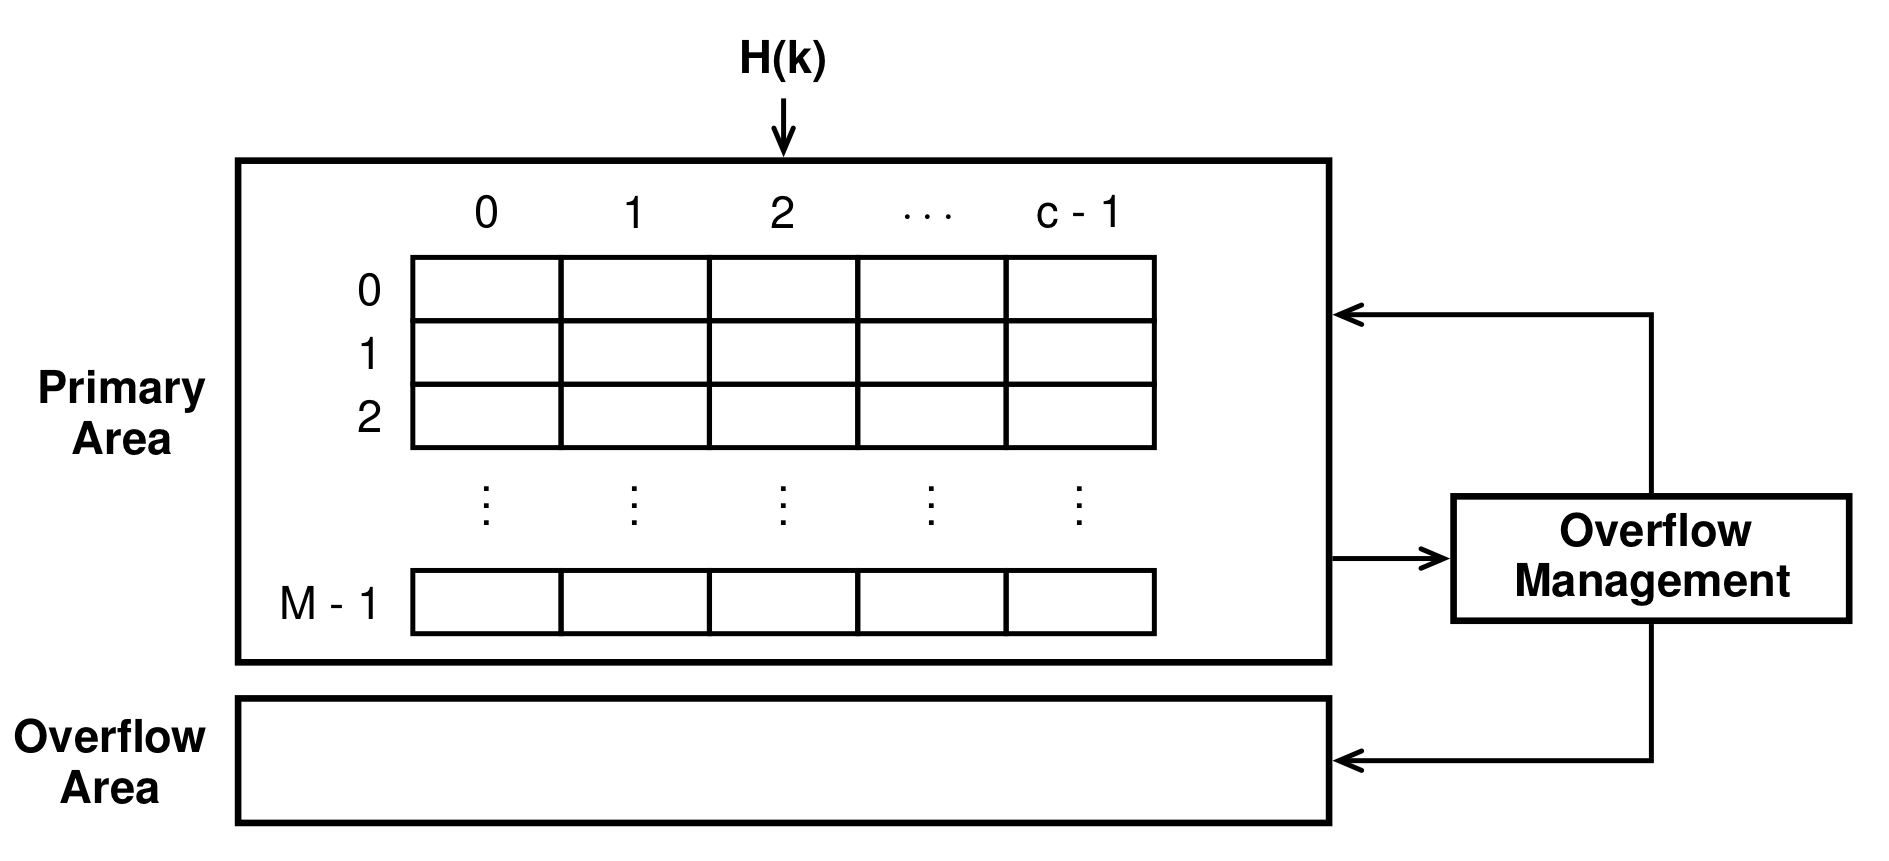
\includegraphics[width=0.7\linewidth]{images/DBMS_Internals/HashingOrganization/static_hashing.jpeg}
    \caption{Static hashing organization}
\end{figure}
\end{itemize}



The design of a static hashing organization requires the specification of the following parameters:
\begin{itemize}
    \item \textbf{Hash Functions}
    \begin{itemize}
        \item The hash function \(H\) is uniform if all the addresses produced are \textbf{uniformly distributed}  in the interval \((0, M-1)\)
        \item Two keys \(k_1\) and \(k_2\) are synonyms if \(H(k_1) = H(k_2)\), that is if they produce a \textbf{collision}
        \item If the number of collisions is greater than the page capacity, there is an \textbf{overflow}. The overflows, during the search, increases the cost of the operation
        \item When it is well designed (80\% page occupancy), we can assume that there are no  overflows and so a record is retrieved with 1 page access.
        \item The typical hash function is the “division method” (Mp is a prime number):
        \[H(k) = k \text{ mod } M_p\]
    \end{itemize}
    \item \textbf{Overflow Manager}
    \begin{itemize}
        \item \textit{Open Overflow} performs a primary area linear search to find the first available page to insert the overflow record. When the last page has been searched, the process starts back
        \item \textit{Chained overflow} inserts the overflow record in another page of a different overflow area
    \end{itemize}
    \item \textbf{Loading Factor} computed as \(d = N/(M \times c)\)
    \begin{itemize}
        \item High loading factor reduces memory size and increases the cost of operation 
        \item Influence of loading factor on average search cost
    \end{itemize}
    \item \textbf{Page Capacity}
    \begin{itemize}
        \item Describe the point in which we start to have overflow, thus it is better to have large capacity
        \item If page capacity increases ,the percentage of overflows decreases 
    \end{itemize}
\end{itemize}

\subsection{Performance Evaluation}
A static hashing organization has excellent performance as long as there are no overflows to manage. Overflows quickly degrade performance and so a reorganization must be performed of the hash structure.
\begin{itemize}
    \item \textbf{Search for single key:} 1 page access
    \item \textbf{Range search:} cannot be performed
    \item \textbf{Insertion:} usually cost 1 page access in case of overflow it will cost 2
    \item \textbf{Deletion} Cost of searching plus writing the page , it costs 2 page access
\end{itemize}
To reduce the cost of data loading, and to improve then performance, the operation proceeds as follow:
\begin{enumerate}
    \item Build a temporary file of pairs: (Record with key \(K_i, H(K_i)\))
    \item  Sort the file on \(H(K)\) 
    \item Load the records in the hash files, in two passes:
    \begin{enumerate}
        \item Load the records which do not overflow
        \item Then load the records which do overflow
    \end{enumerate}
\end{enumerate}
The \textbf{reorganization} of the hash file is obtained by copying the records in an auxiliary file and then doing a loading. It is needed when:
\begin{itemize}
    \item When the overflow percentage is high
    \item When the file has a high volatility, to reuse the space of logical deletions
\end{itemize}

\section{Dynamic Hashing Organizations}
Several dynamic hashing organizations have been proposed to avoid the reorganization which is necessary in static hashing organizations. Dynamic hashing can be summarize with two groups:
\begin{itemize}
    \item \textbf{With auxiliary data structures:} \textit{virtual hash, extensible hash, dynamic hash}
    \item \textbf{Without auxiliary data structures:} \textit{linear hash, spiral hash}
\end{itemize}

\subsection{Virtual hashing}
Virtual hashing works as follow:
\begin{itemize}
    \item The data area contains initially \(M\) contiguous pages with a capacity of \(c\) records. A page is identified by its address, a number between \(0\) and \(M - 1\).
    \item A bit vector \(\beta\) is used to indicate with a 1 which page of the data area contains at least a record.
    \item  Initially a hashing function \(H_0\) is used in order to map each key value \(k\) to an address \(m = H_0(k)\), between \(0\) and \(M - 1\) where the record with the key \(k\) should be stored. If an overflow is generated then:
    \begin{itemize}
        \item The data area is doubled
        \item The hashing function \(H_0\) is replaced by the new hashing function \(H_1\) that produces page addresses between \(0\) and \(2M - 1\)
        \item The hashing function \(H_1\) is applied to \(k\) and all the records of the original overflowing page \(m\) to distribute the records between \(m\) and a new page \(m'\) in the new half of the table.
    \end{itemize}
\end{itemize}

This method requires the use of a hashing functions series \(H0, H1, H2, ..., Hr\); in general, Hr produces a page address between \(0\) and \(2^rM - 1\). The index of the hashing function H is the number of times that the data area has been doubled.

The function suggested by Litwin is:
\[H_r(k) = k\text{ mod }(2^r \times M)\]
Where
\begin{itemize}
    \item \(k\) is the key of a record to be retrieved
    \item \(r\) is the number of doubling of the data area.
\end{itemize}

\begin{figure}[!h]
    \centering
    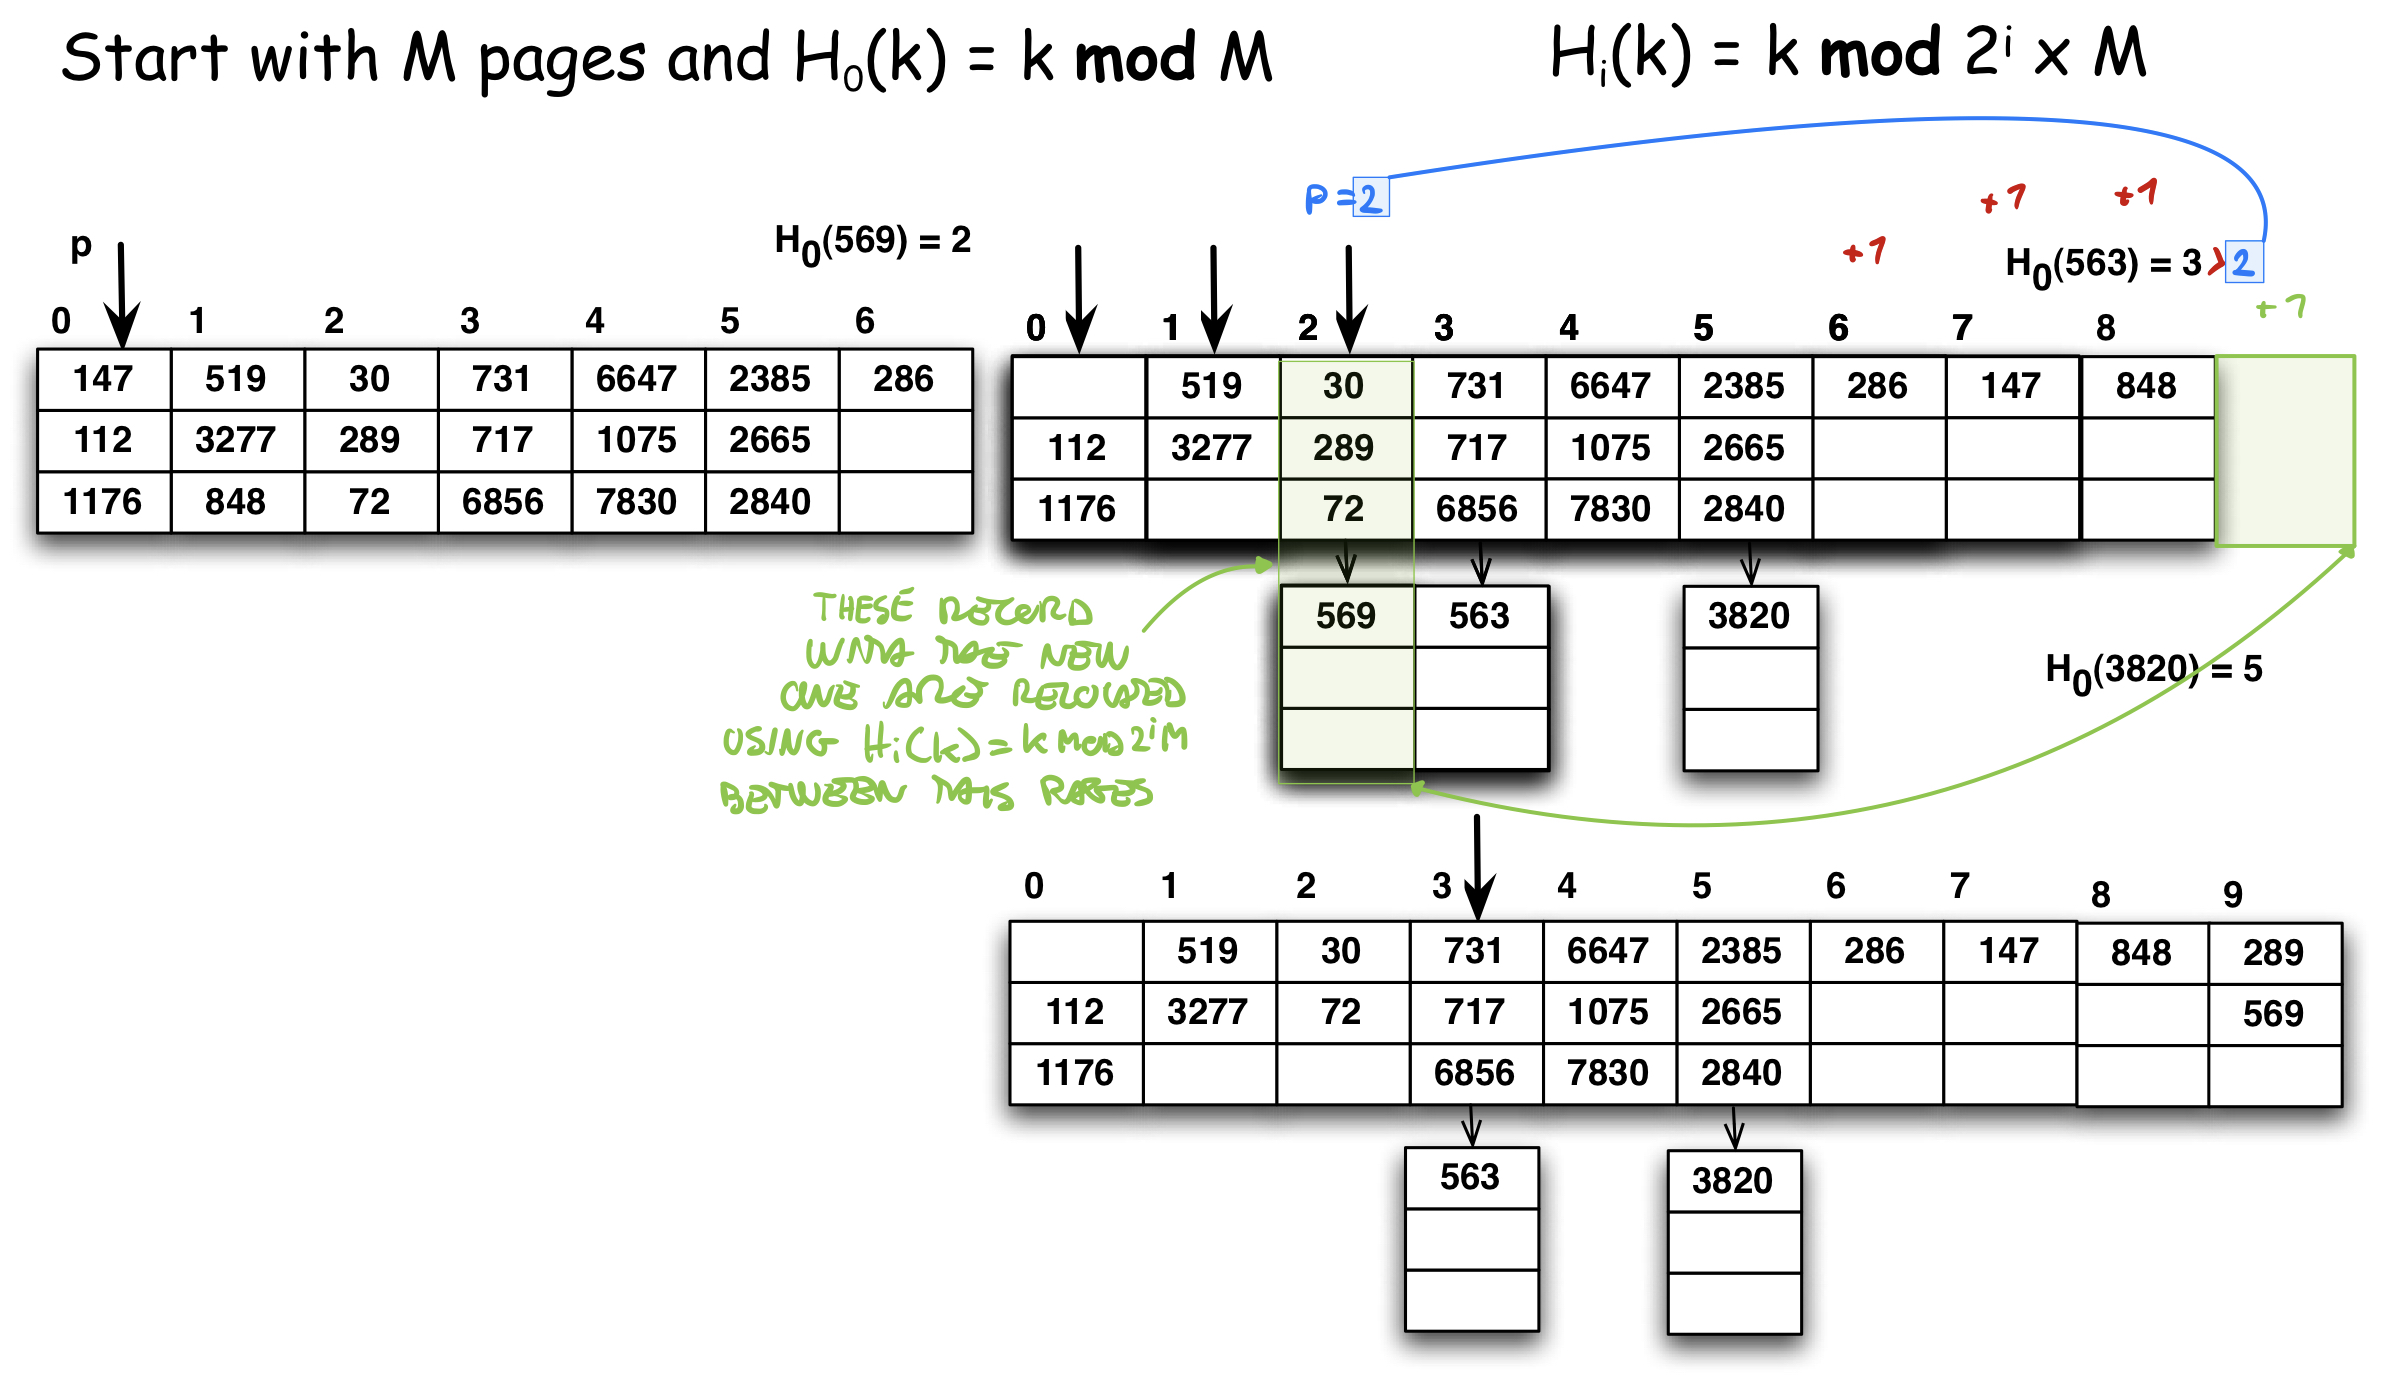
\includegraphics[width=0.8\linewidth]{images/DBMS_Internals/HashingOrganization/virtual_hashing.jpeg}
    \caption{Example of Virtual Hashing}
\end{figure}

\begin{figure}[!h]
    \centering
    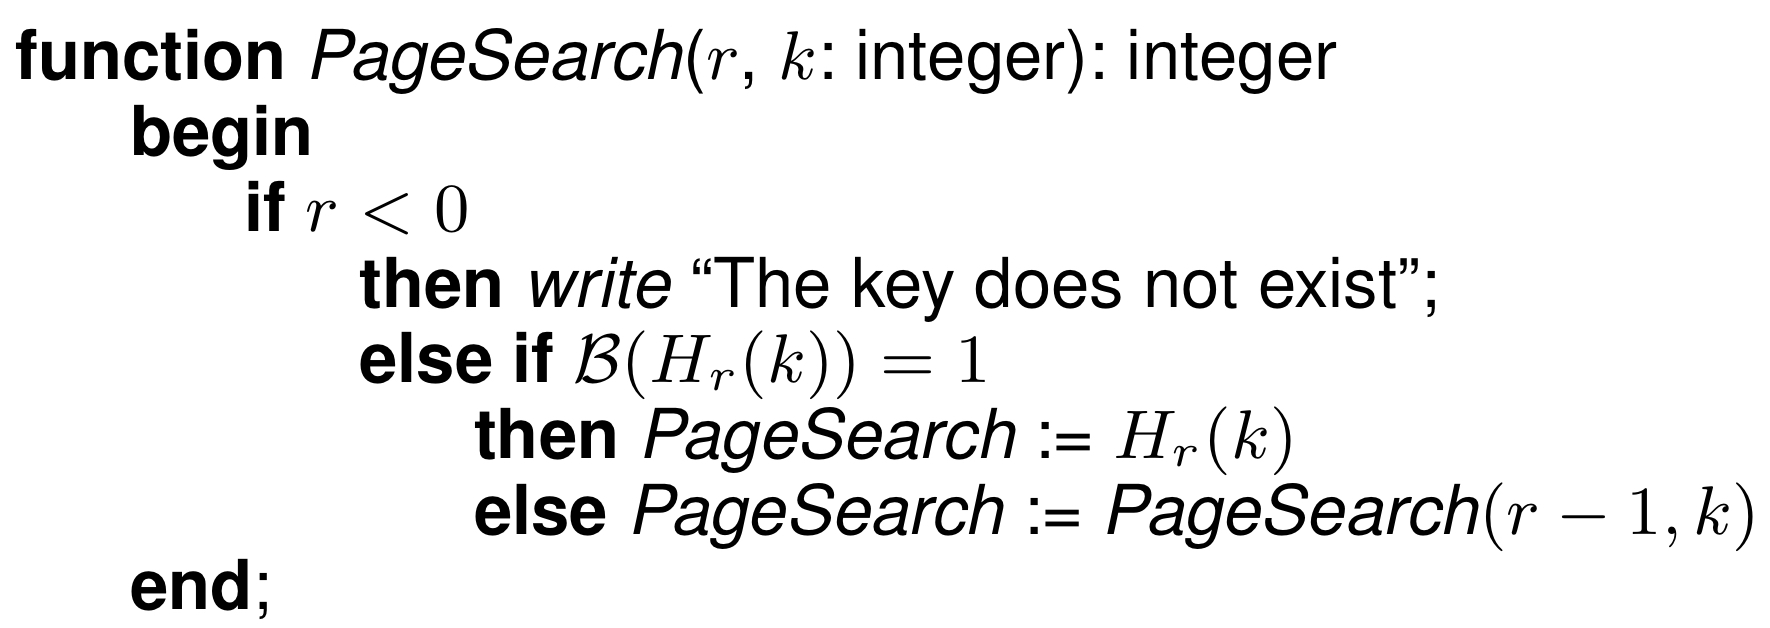
\includegraphics[width=0.5\linewidth]{images/DBMS_Internals/HashingOrganization/search_operation.jpeg}
    \caption{Search operation}
\end{figure}






\subsection{Linear Hashing}
\begin{itemize}
    \item The idea of this method is again to increase the number of data pages as soon as a page overflows
    \item The page which is split is not the one that flows over, but the page pointed by the current pointer \(p\), initialized to the first page \((p = 0)\) and incremented by 1 each time a page is split.
\end{itemize}
The process is like so:
\begin{enumerate}
    \item \(M\) pages are allocated and the hash function is \(H_0(k) = k \text{ mod } M\)
    \item When there is an overflow from a page with address \(m \geq p\) an overflow chain is maintained for the page \(m\), but a new page is added
    \item The records in page \(p\), and possible overflows from this page, are distributed between the page \(p\) and the new page using the hash function \(H_1(k) = k \text{ mod } 2M\) which generates addresses between \(0\) and \((2M - 1)\) 
    \begin{figure}[!h]
    \centering
    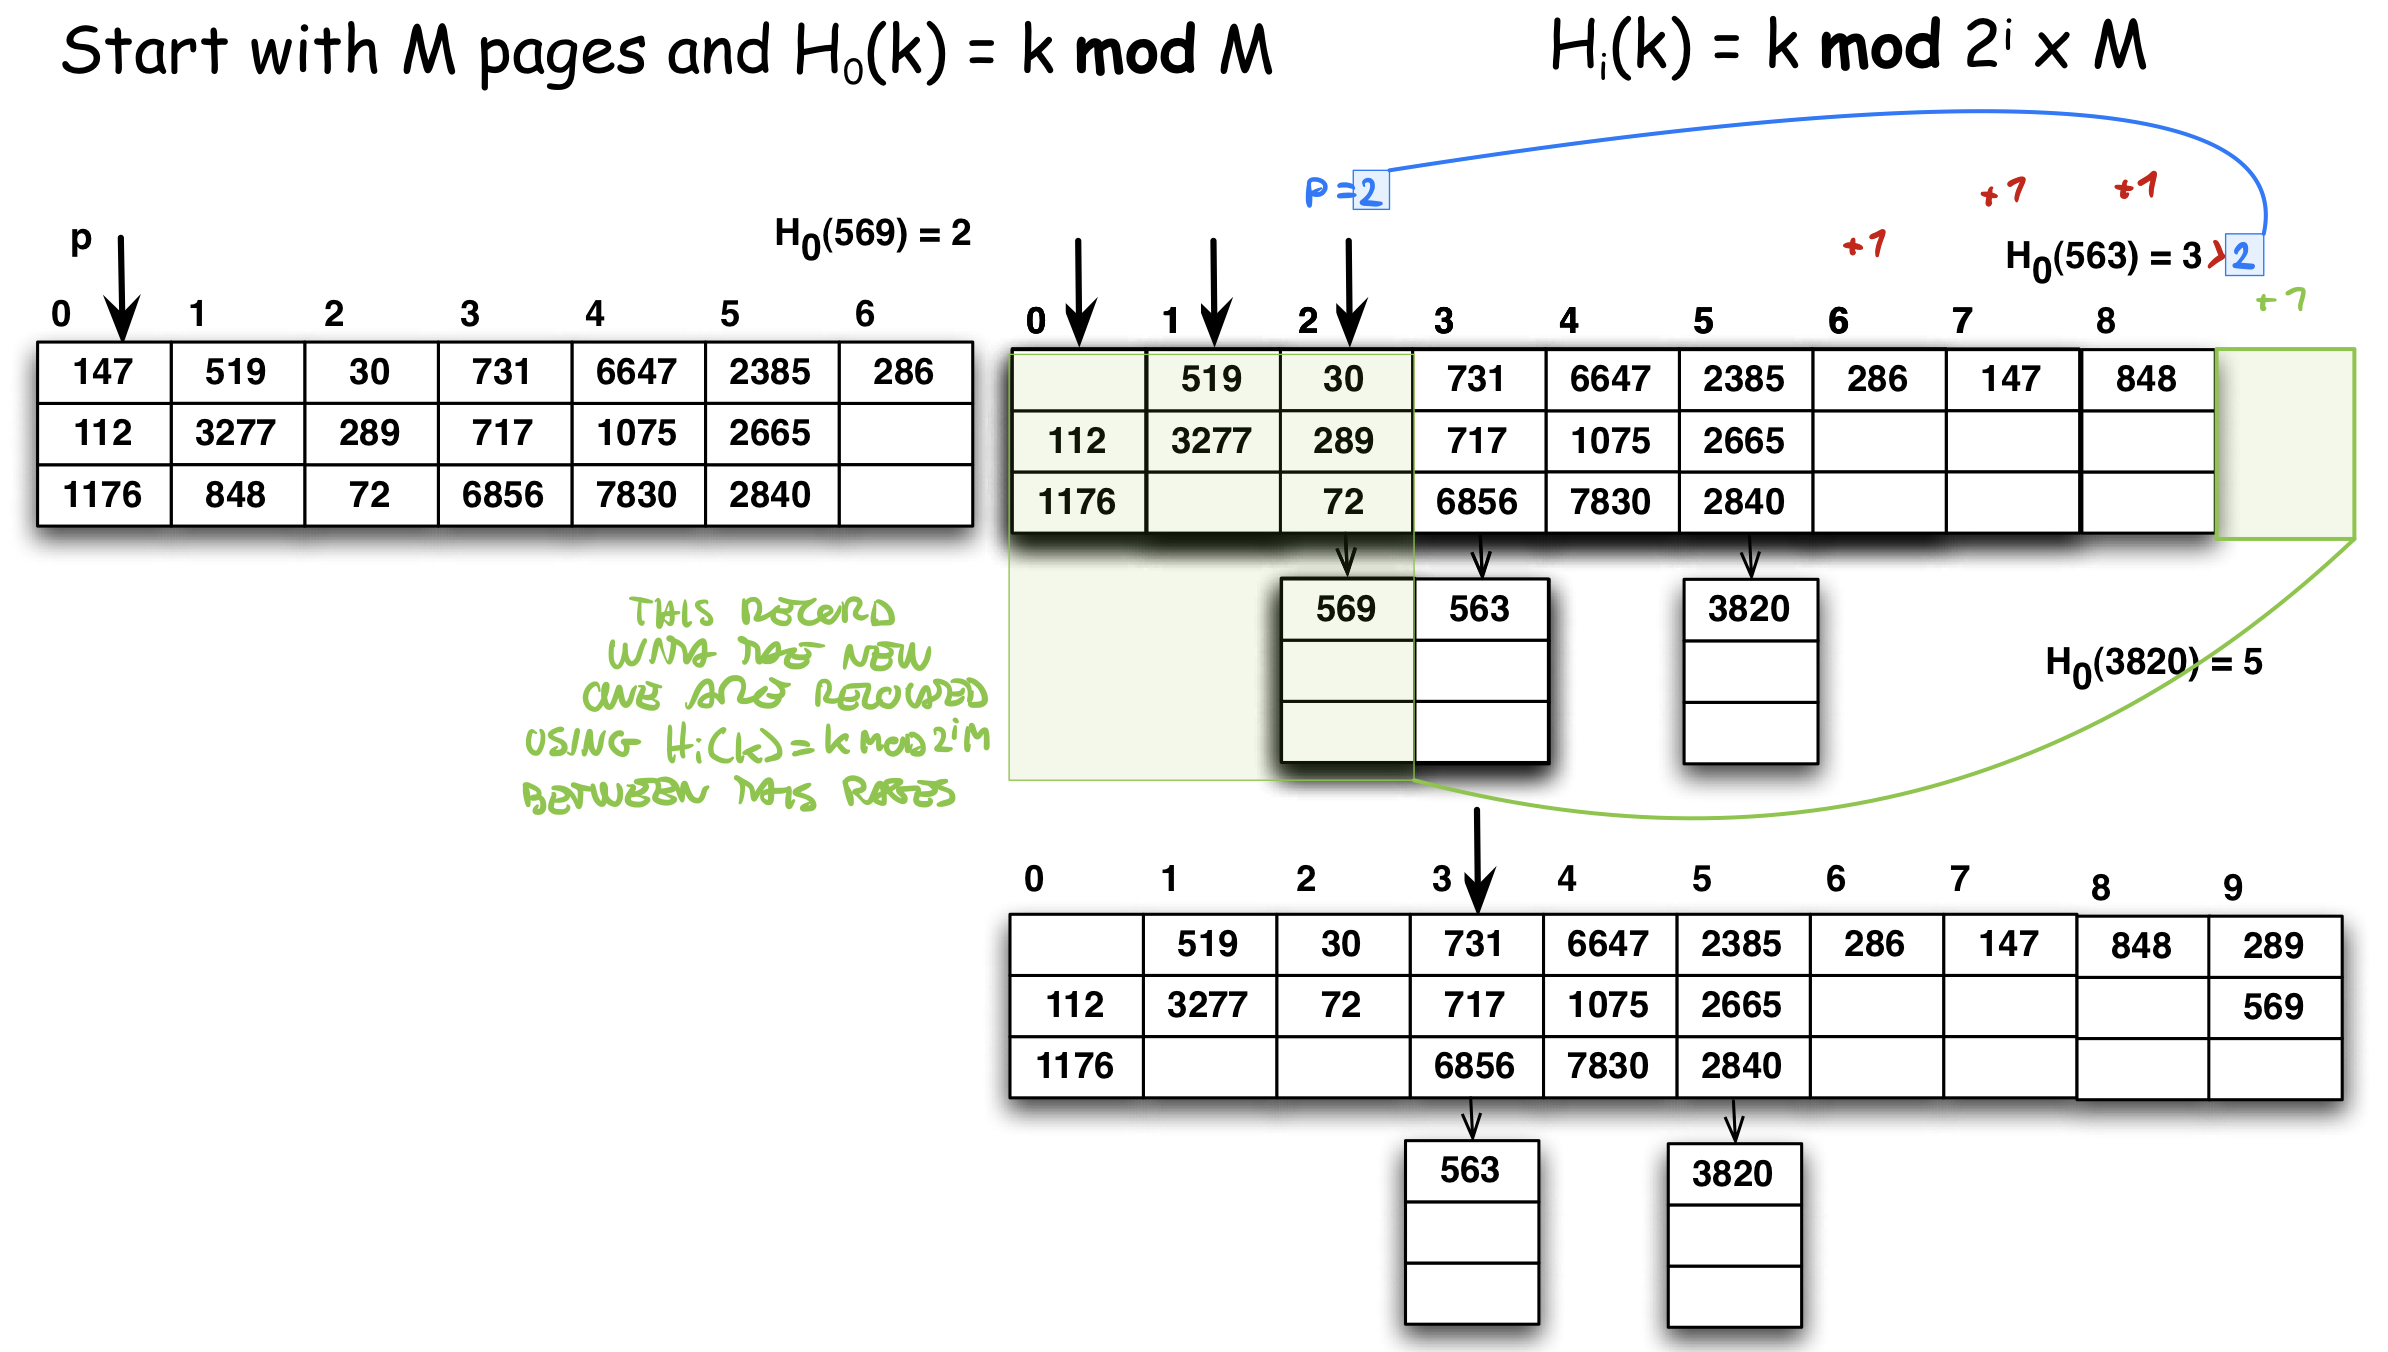
\includegraphics[width=0.8\linewidth]{images/DBMS_Internals/HashingOrganization/linear_hashing.jpeg}
    \caption{Example of Linear Hashng}
\end{figure}

\end{enumerate}
